%==============================================================================
% presentation.tex
%==============================================================================


%==============================================================================
% Configuration
%==============================================================================

% Internationalisation
\usepackage[utf8]{inputenc}
\usepackage[T1]{fontenc}
% \usepackage[ngerman]{babel}

% Miscellaneous packages
\usepackage{url}
\usepackage{color,listings,paralist}
\usepackage{enumerate}
\usepackage{tabularx}
\usepackage{alltt}
\usepackage{wasysym}
\usepackage{numprint}

% Use default Acrobat reader fonts
\usepackage{mathpazo}

% Use CM fonts (increases document size)
\usepackage{ae}

% Use images
\usepackage{graphicx}

% Configure beamer
\usetheme[secheader]{Ikhono}
\usefonttheme[onlylarge]{structurebold}
\setbeamertemplate{navigation symbols}{}

% Variables
\providecommand{\Title}{An Advanced Scheduler for Intervals}
\providecommand{\Subtitle}{Master's Thesis}
\providecommand{\Author}{Thomas Weibel <weibelt@ethz.ch>}
\providecommand{\Institute}{Laboratory for Software Technology, \\
  Swiss Federal Institute of Technology Z\"urich}
\providecommand{\Date}{September 7, 2010}

% PDF settings
\hypersetup{
  pdftitle={\Title, \Subtitle},
  pdfauthor={\Author},
  pdfsubject={\Institute},
  pdfkeywords={Master's Thesis, Thomas Weibel, Intervals, Parallel Programming}
}

% Titlepage
\title{\Title}
\subtitle{\Subtitle}
\author{\Author}
\institute{\Institute}
\date{\Date}

% Listings
\lstdefinestyle{Default}{
  language=Java,
  tabsize=2,
  mathescape=true,
  inputencoding=utf8,
  showstringspaces=false,
  fontadjust=true,
  basicstyle=\ttfamily,
  keywordstyle=\color{blue}\bfseries,
}
\lstset{style=Default}


%==============================================================================
% Document
%==============================================================================

\begin{document}


% Titlepage
\begin{frame}[plain]
  \titlepage
\end{frame}

\note{
  \begin{itemize}
  \item Hi and welcome to my talk.
  \item I'm going to present the work from my Master's thesis. The
    topic was ``Advanced Scheduling for Intervals''.
  \end{itemize}
}


\section*{Introduction}

\begin{frame}{Executive Summary}
  \begin{itemize}
  \item Advanced work-stealing scheduler for intervals
    \begin{itemize}
    \item[$\rightarrow$] Locality-aware scheduling using locality
      hints provided by the programmer
    \end{itemize}
  \item Providing locality hints to intervals is optional
    \begin{itemize}
    \item[$\rightarrow$] Performance of locality-ignorant programs
      executed with new scheduler implementation comparable to
      original scheduler
    \end{itemize}
  \item Locality hints improve runtime and cache hit and miss rates
    \begin{itemize}
    \item[$\rightarrow$] \emph{Best locality} placement achieves up to
      $1.15\times$ speedup
    \item[$\rightarrow$] Cache hits increase by $1.5\times$ and cache
      misses decrease by $3.1\times$
    \end{itemize}
  \end{itemize}
\end{frame}

\note{ 
  \begin{itemize}
  \item We implement and analyze an advanced scheduler for intervals
    which is designed for locality-aware scheduling using locality
    hints provided by the programmer.
  \item Providing locality hints is optional and the performance of
    locality-ignorant programs executed with the new scheduler
    implementation is comparable to that of the original scheduler.
  \item We studied the performance of our new scheduler implementation
    with benchmarks using data sharing intervals. The experimental
    results show that \emph{best locality} placement of intervals
    achieves up to 15 percent speedup while cache hits are increased
    and cache misses reduced.
  \end{itemize}
}

\begin{frame}{Work-Stealing Intervals Scheduler}
  \begin{itemize}
  \item Employs a fixed number of worker threads
  \item Each worker has local deque to maintain its own pool of ready
    intervals:
    \begin{itemize}
    \item Puts and takes intervals to execute at the tail of its deque
    \item When its deque is empty, tries to steal an interval from the
      deque's head of a victim worker chosen at random
    \end{itemize}
  \item Reduces contention by having owner and thieves working on
    opposite sides of the deque
    \begin{itemize}
    \item Owner manipulates its deque in a LIFO (stack-like) manner
    \item Stealing operates in a FIFO manner
    \end{itemize}
  \end{itemize}
\end{frame}

\note{
  \begin{itemize}
  \item The implementation of intervals makes use of a work-stealing
    scheduler similar to those found in Cilk or Java 7. The intervals
    scheduler employs a fixed number of threads called workers.
  \item Each worker has a local deque to maintain its own pool of
    ready intervals:
    \begin{itemize}
    \item When assigning a new interval to a worker, the worker puts
      it onto the tail of its deque. And when obtaining work, it takes
      a ready interval from the tail of its deque to execute.
    \item When a worker's deque is empty, it tries to steal an
      interval from the deque's head of a victim worker chosen at
      random.
    \end{itemize}
  \item Work-stealing scheduling reduces contention by having owner
    and thieves working on opposite sides of the deque: 
    \begin{itemize}
    \item As long as a worker's deque is not empty, the worker
      manipulates its deque in a stack-like manner.
    \item And since steals take place at the head of the victim's
      deque, stealing operates in a FIFO manner.
    \end{itemize}
  \end{itemize}
}

\begin{frame}{Locality-Aware Intervals Scheduling}
  \begin{itemize}
  \item Modern CMPs feature heterogeneous memory hierarchies:
    \begin{itemize}
    \item Access times depend on which processor interval is running
    \item May be better to run interval on one processor than another
    \end{itemize}
  \item Locality-aware intervals can lead to improved performance:
    \begin{itemize}
    \item Data sharing intervals running on the same processor perform
      prefetching of shared regions for one another
    \item Running non-communicating intervals with high memory
      footprints on different processors reduces cache contention
    \end{itemize}
  \item Current work-stealing intervals scheduler is locality-ignorant
  \end{itemize}

  \begin{itemize}
  \item[$\Rightarrow$] Introduce LASSI\footnote{The correct acronym
      would be LASI but we chose LASSI instead as we really enjoy
      drinking refreshing masala lassi \smiley}, a locality-aware
    scheduler for intervals
  \end{itemize}
\end{frame}

\note{
  \begin{itemize}
  \item As modern chip multiprocessor systems feature a heterogeneous
    memory hierarchy where access times depend on which processor an
    interval is running, it may be more efficient to schedule an
    interval on one processor than another.
  \item Locality-aware intervals can lead to improved performance:
    \begin{itemize}
    \item By scheduling data sharing intervals on the same processor
      they perform prefetching of shared regions for one another.
    \item Scheduling non-communicating intervals with high memory
      footprints on different processors helps to reduce cache
      contention and potential cache capacity problems.
    \end{itemize}
  \item The current implementation of the intervals library uses a
    locality-ignorant work-stealing scheduler to schedule ready-to-run
    intervals.
  \item Thus, we implement and analyze LASSI, a locality-aware
    scheduler for intervals.
  \end{itemize}
}


\section{Approach}

\begin{frame}{Outline}
  \tableofcontents[current]
\end{frame}

\note{
  \begin{itemize}
  \item Before starting with the implementation of the new scheduler,
    we implement a synthetic multi-threaded locality-aware benchmark
    called \emph{Cache Stress Test}.
  \item This benchmark serves as a proof of concept for our plan to
    introduce locality-aware intervals.
  \end{itemize}
}

\begin{frame}{Cache Stress Test}
  \begin{columns}[c]
    \begin{column}{0.47\textwidth}
      \begin{itemize}
      \item Randomly initializes two integer arrays of size 8 MB
      \item Binds 8 \emph{Cache Stress} threads to each core
      \item Half of the threads work with array 0, the other half with
        array 1
      \item Each thread adds and multiplies all the elements of its
        array 100 times
      \end{itemize}
    \end{column}
    \begin{column}{0.53\textwidth}
      \begin{center}
        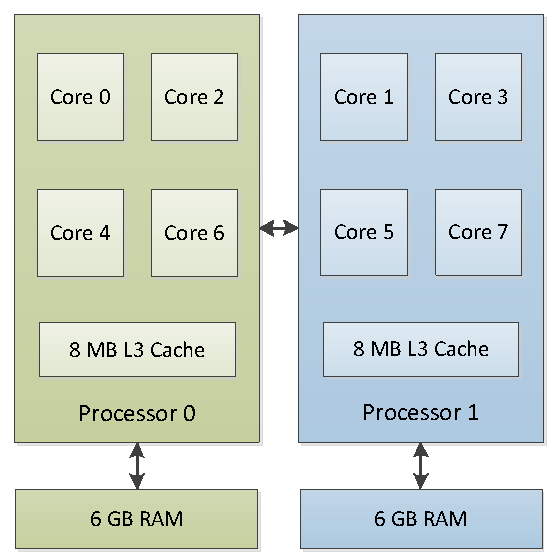
\includegraphics[width=\textwidth]{figures/mafushi} \\
        \tiny{Intel Nehalem test system}
      \end{center}
    \end{column}
  \end{columns}
\end{frame}

\note{
  \begin{itemize}
  \item We wrote our benchmark for ``mafushi'', our Intel Nehalem
    system. ``mafushi'' has 2 processors with 4 cores each. The two 8
    MB L3 caches are shared between all cores of the same processor.
  \item \emph{Cache Stress Test} first randomly initializes two
    integer arrays of size 8 MB.
  \item Then the benchmark creates 8 \emph{Cache Stress} threads per
    core with their affinity set to this specific core.
  \item One half of the threads operate on the elements of the first
    array and the other half operate on the elements of the second
    array.
  \item Each thread adds and multiplies all the elements of its
    respective array 100 times.
  \end{itemize}
}

\begin{frame}{Best and Worst Locality}
  \begin{columns}[c]
    \begin{column}{0.50\textwidth}
      \begin{center}
        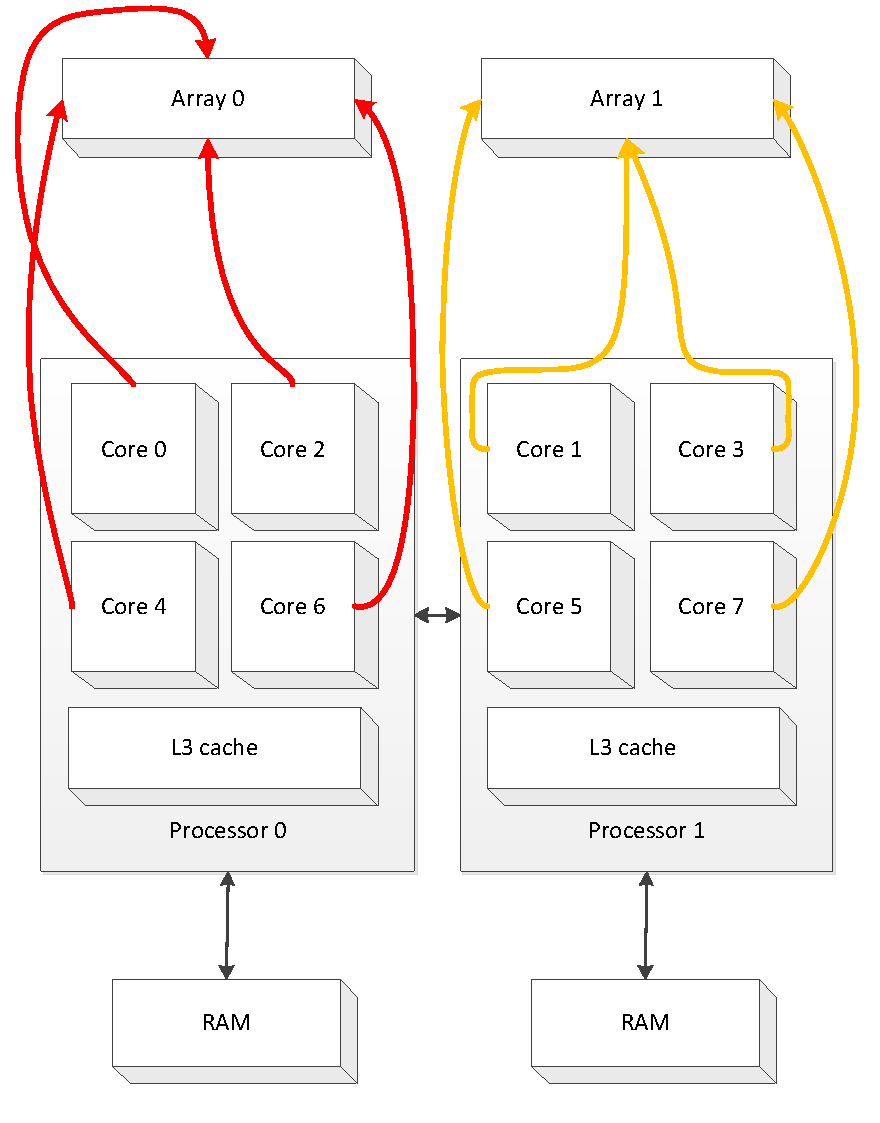
\includegraphics[width=\textwidth]{figures/cache-stress-test-mafushi-threads-best} \\
        \tiny{Best locality}     
      \end{center}
    \end{column}
    \begin{column}{0.50\textwidth}
      \begin{center}
        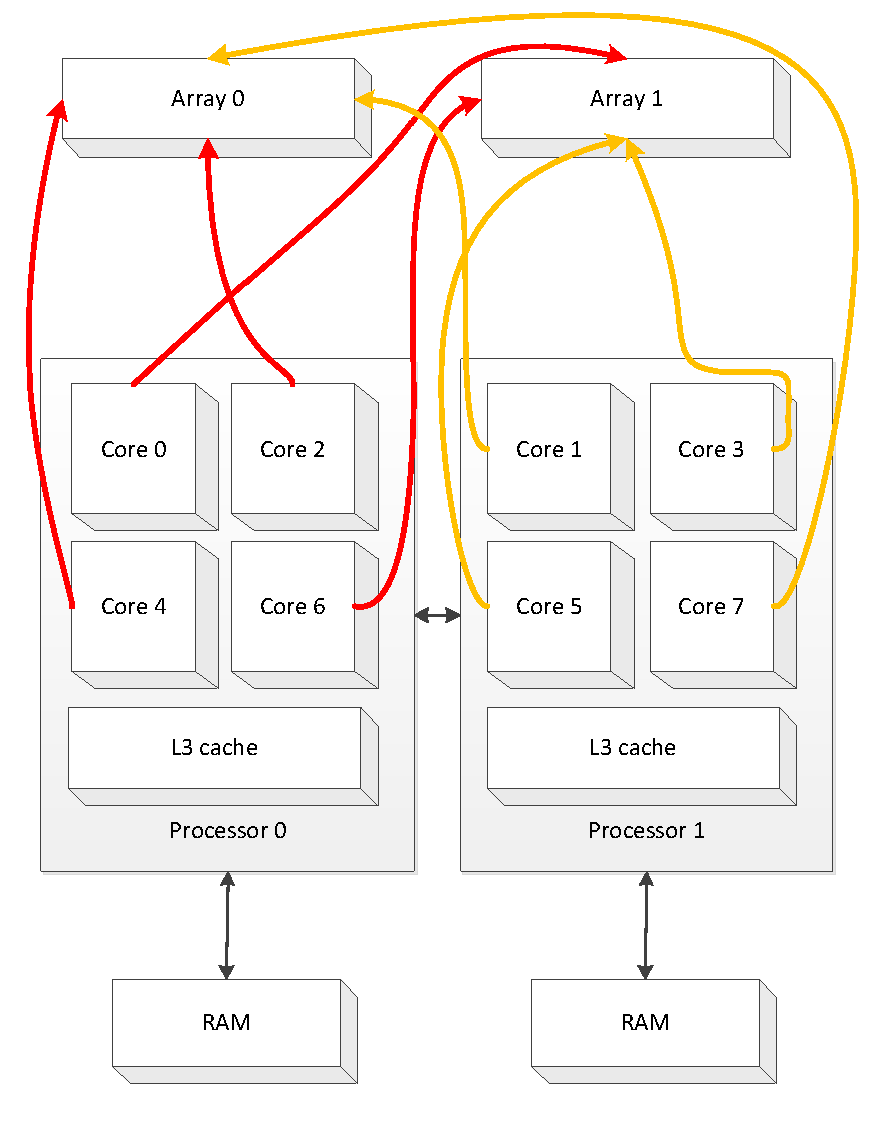
\includegraphics[width=\textwidth]{figures/cache-stress-test-mafushi-threads-worst} \\
        \tiny{Worst locality}
      \end{center}
    \end{column}
  \end{columns}
\end{frame}

\note{
  We implement several different variants of the \emph{Cache Stress
    Test}, each having different locality properties.

  \begin{itemize}
  \item In the \emph{Best Locality} implementation all the threads
    working on the first array have affinity for a core on the first
    processor and all threads working on the second array have
    affinity for a core on the second processor.
  \item When using \emph{Worst Locality}, half the threads with
    affinity for a core on the first processor work on the first
    array, and the other half work on the second array and vice versa.
  \end{itemize}
  
  Besides \emph{Best} and \emph{Worst Locality} we also implement
  variants with \emph{Ignorant} and \emph{Random Locality}.
}

\begin{frame}{Execution Times}
  \begin{columns}[c]
    \begin{column}{0.49\textwidth}
      \begin{itemize}
      \item \emph{Best locality} variant: Sharing threads run on same
        processor $\rightarrow$ perform prefetching of array elements
        for each other
      \item Other variants: Threads compete for L3 caches
      \item \emph{Best locality} has significant speedup of up to
        $1.55\times$
  \end{itemize}
    \end{column}
    \begin{column}{0.51\textwidth}
      \begin{center}
        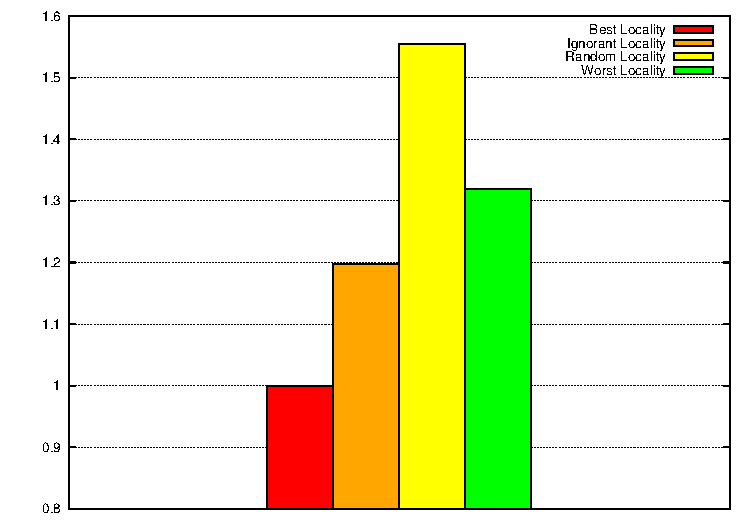
\includegraphics[width=\textwidth]{figures/cache-stress-test-threads} \\
        \tiny{Execution times normalized to \emph{best locality}}
      \end{center}
    \end{column}
  \end{columns}
\end{frame}

\note{
  \begin{itemize}
  \item When we are using the \emph{best locality} variant, we move
    all sharing threads onto the same processor which will perform
    prefetching of the array elements for each other.
  \item The exact opposite happens in the other variants: Threads
    compete for the L3 caches.
  \item The \emph{best locality} implementation shows a significant
    speedup over the other locality benchmarks of 20 to 55 percent.
  \end{itemize}
}

\begin{frame}{Cache Read Hits and Misses}
  \begin{itemize}
  \item \emph{Best locality} benchmark has between $1.5\times$ and
    $1.8\times$ more L3 cache read hits, and between $3.6\times$ and
    $4.5\times$ fewer read misses
  \item Cache read hits and misses normalized to the \emph{best
      locality} implementation:
  \end{itemize}
  
  \vspace{\stretch{1}}

  \begin{columns}[c]
    \begin{column}{0.50\textwidth}
      \begin{center}
        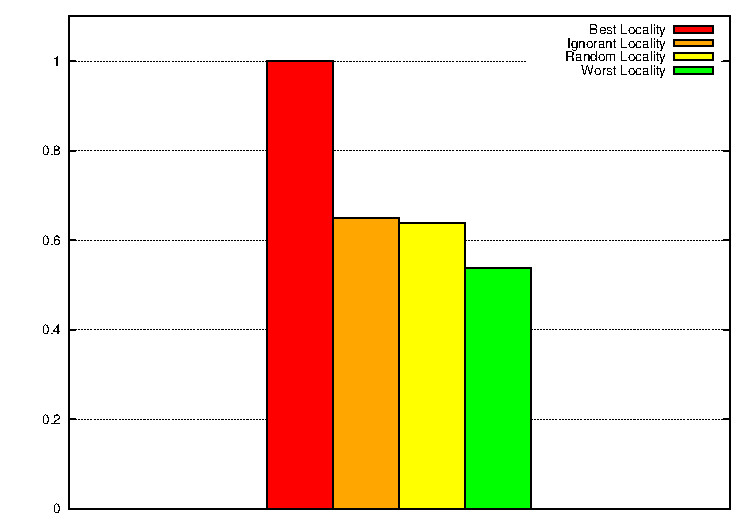
\includegraphics[width=\textwidth]{figures/cache-stress-test-threads-cache-hits} \\
        \tiny{Cache read hits}     
      \end{center}
    \end{column}
    \begin{column}{0.50\textwidth}
      \begin{center}
        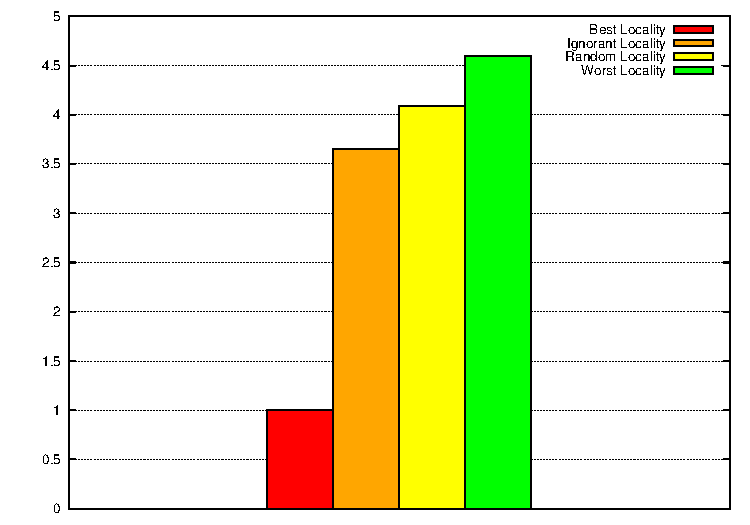
\includegraphics[width=\textwidth]{figures/cache-stress-test-threads-cache-misses} \\
        \tiny{Cache read misses}
      \end{center}
    \end{column}
  \end{columns}
\end{frame}

\note{
  \begin{itemize}
  \item Compared to the other benchmarks, the \emph{best locality}
    benchmark has between 50 and 80 percent more L3 cache read hits,
    and between 360 and 450 percent fewer cache read misses.
  \item The figure shows them normalized to the measurements of the
    \emph{best locality} implementation.
  \end{itemize}
}


\section{Implementation}

\begin{frame}{Outline}
  \tableofcontents[current]
\end{frame}

\note{
  \begin{itemize}
  \item Our experiments confirmed the hypothesis that the locality of
    threads matters.
  \item Thus, we decided to rewrite the intervals scheduler to support
    locality hints provided by the programmer.
  \end{itemize}
}

\subsection{Locality-Aware Intervals}

\begin{frame}[fragile]{Locality-Aware Intervals API}
  \begin{itemize}
  \item Intervals are subtypes of abstract class \lstinline!Interval!
  \item Specify the interval's locality when creating it
  \item Locality hints provided in the form of \lstinline!PlaceID!
    objects
    \begin{itemize}
    \item[$\rightarrow$] Assign the interval to the specified place
    \end{itemize}
  \item If \lstinline!PlaceID! is null, the interval is ignorant of
    its place    
    \begin{itemize}
    \item[$\rightarrow$] Assign the interval to a place in a
      round-robin fashion
    \end{itemize}
  \end{itemize}

  \vspace{\stretch{1}}

\begin{lstlisting}[basicstyle=\fontsize{8}{10}\selectfont\ttfamily]
  public abstract class Interval extends WorkItem {	
    public final PlaceID place;

    public Interval(Dependency dep, String name, PlaceID place) {
      this.place = place;  
      // ...
    }
    
    // ...
  }\end{lstlisting}
\end{frame}

\note{
  \begin{itemize}
  \item Intervals are represented as subtypes of the abstract class
    \lstinline!Interval!.
  \item To make an interval locality-aware, the programmer has to
    specify the interval's locality when creating it. We extend the
    abstract \lstinline!Interval! class to support locality hints.
  \item Locality hints are provided in the form of \lstinline!PlaceID!
    objects. They specify which place the interval should be executed
    on.
  \item If the interval should be ignorant of its place, the
    programmer can provide \lstinline!null! when creating it. This
    makes the scheduler to assign the interval to a place in a
    round-robin fashion.
  \end{itemize}
}

\subsection{Work-Stealing Places}

\begin{frame}{Work-Stealing Places}
  \begin{itemize}
  \item Traditional work-stealing scheduler designs: Every worker has
    local deque to maintain own pool of ready tasks
  \item LASSI uses \emph{Work-Stealing Places} instead:
    \begin{itemize}
    \item Each place has a fixed number of workers and a local deque
    \item Workers of a place share its local deque
    \item When the pool of a place is empty, its workers tries to
      steal a task from the pool of a victim place chosen at random
    \end{itemize}
  \end{itemize}
\end{frame}

\note{
  \begin{itemize}
  \item In traditional work-stealing scheduler designs, every worker
    has a local deque, to maintain its own pool of ready tasks from
    which it obtains work.
  \item LASSI uses \emph{Work-Stealing Places} instead:
    \begin{itemize}
    \item Each work-stealing place has a fixed number of workers and a
      local deque to maintain ready tasks.
    \item The workers of a place share its local deque from which they
      obtain work.
    \item When a worker finds that the pool of its place is empty, it
      tries to steal a task from the pool of a victim place chosen at
      random.
    \end{itemize}
  \end{itemize}
}

\begin{frame}{Intel Nehalem in Two-Processor Configuration}
  \begin{center}
    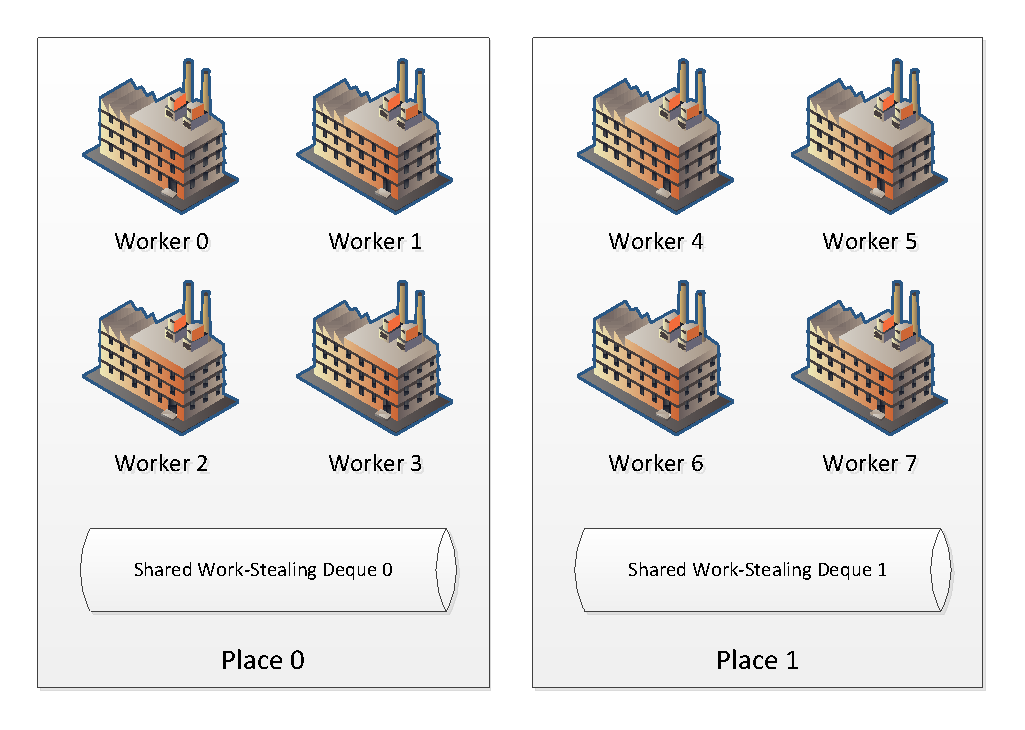
\includegraphics[width=0.93\textwidth]{figures/places} \\
    \tiny{\emph{Work-Stealing Places} used in our Intel Nehalem
      testing machine}
  \end{center}
\end{frame}

\note{
  \begin{itemize}
  \item The figure shows the work-stealing places used on our Intel
    Nehalem testing machine.
  \item Places are virtual: The mapping of physical units to places is
    performed by a concrete implementation of the abstract
    \lstinline!Places! class.
  \item For our test machine we define a place for each processor.
  \end{itemize}
}

\begin{frame}{Alternative Designs}
  \begin{itemize}
  \item Other designs provide each worker with mailbox in addition to
    work-stealing deque:
    \begin{itemize}
    \item Worker pushes work item onto both its deque and into the
      mailbox of the worker the item has affinity for
    \item Worker tries to get work from its mailbox before stealing
    \item Work items must be idempotent as they can appear twice
    \end{itemize}
  \item Simplify by using a shared deque per \emph{Work-Stealing
      Place}
  \item Will not impact scalability as long as the places are small
    \begin{itemize}
    \item[$\rightarrow$] Up to 8 workers: No significant difference
      between using separate deque for each worker or shared deque per
      place
    \end{itemize}
  \end{itemize}
\end{frame}

\note{
  \begin{itemize}
  \item Other locality-aware work-stealing schedulers provide each
    worker with a mailbox in addition to the work-stealing deque:
    \begin{itemize}
    \item When creating a work item, a worker will push it onto both
      its deque and also into the tail of the mailbox of the worker
      that the interval has affinity for.
    \item A worker will first try to obtain work from its mailbox
      before attempting to steal.
    \item Because work items can appear twice, once in a mailbox and
      once in a deque, they have to be idempotent.
    \end{itemize}
  \item We have decided to simplify our scheduler implementation by
    using a shared deque per \emph{Work-Stealing Place}.
  \item This will not impact scalability as long as the places are not
    too large. We could show that up to 8 workers there is no
    significant difference between using a separate deque for each
    worker or a shared deque per place.
  \end{itemize}
}

\begin{frame}{Setting Core Affinity of Worker Threads}
  \begin{columns}[c]
    \begin{column}{0.62\textwidth}
      \begin{itemize}
      \item 1-to-1 correspondence between Java and native threads
      \item Java Threads API does not expose ability to set the CPU or
        core affinity
      \item JNI library to bind workers to a core:
        \begin{itemize}
        \item \lstinline!pthread_self()! gets the native thread ID
        \item \lstinline!pthread_setaffinity_np()! sets core affinity
          of worker thread
        \end{itemize}
      \end{itemize}
    \end{column}
    \begin{column}{0.38\textwidth}
      \begin{center}
        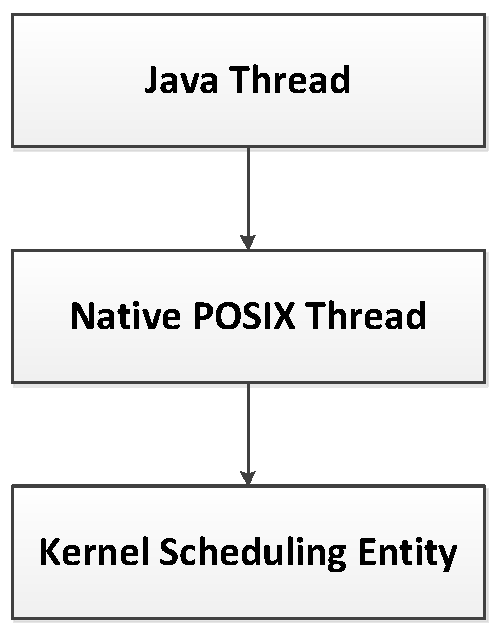
\includegraphics[width=\textwidth]{figures/java-threads} \\
        \tiny{Linux 1-to-1 thread mapping}
      \end{center}
    \end{column}
  \end{columns}
\end{frame}

\note{
  \begin{itemize}
  \item In recent Java Virtual Machines, threads are implemented with
    native threads. This means there is a 1-to-1 correspondence
    between Java and native threads.
  \item Unfortunately the Java Threads API does not expose the ability
    to set the CPU or core affinity despite numerous use cases where
    it would be beneficial such as improving cache and network
    performance or real-time applications.
  \item So to bind the workers to a specific core, we wrote a small
    JNI library.
  \end{itemize}
}

\begin{frame}{Data Locality}
  Setting core affinity of threads only controls locality of work

  \begin{itemize}
  \item[$\rightarrow$] No control over data locality
  \end{itemize}

  \vspace{\stretch{1}}

  \begin{block}{Java HotSpot VM: NUMA-aware allocator}
    \begin{itemize}
    \item Provides automatic memory placement optimizations
    \item Relies on a hypothesis that thread allocating an object will
      be the most likely to use it
      \begin{itemize}
      \item[$\rightarrow$] Places it in the region local to the
        allocating thread
      \end{itemize}
    \item Enabled by invoking the JVM with \lstinline!-XX:+UseNUMA!
  \end{itemize}    
  \end{block}
\end{frame}

\note{
  \begin{itemize}
  \item By setting the core affinity of threads, we only control the
    locality of the work but we do not have control over data
    locality.
  \item In the Java HotSpot VM, the NUMA-aware allocator has been
    implemented to provide automatic memory placement optimizations
    for Java applications.
  \item To enable the NUMA-aware allocator, we invoke the JVM with the
    option \lstinline!UseNUMA! when using LASSI.
  \end{itemize}
}


\section{Performance Evaluation}

\begin{frame}{Outline}
  \tableofcontents[current]
\end{frame}

\note{}

\subsection{Non-Locality Benchmarks}

\begin{frame}{Java Grande Forum Benchmarks}
  New scheduler implementation does not affect performance of existing
  locality-ignorant intervals applications:

  \vspace{\stretch{1}}

  \begin{center}
    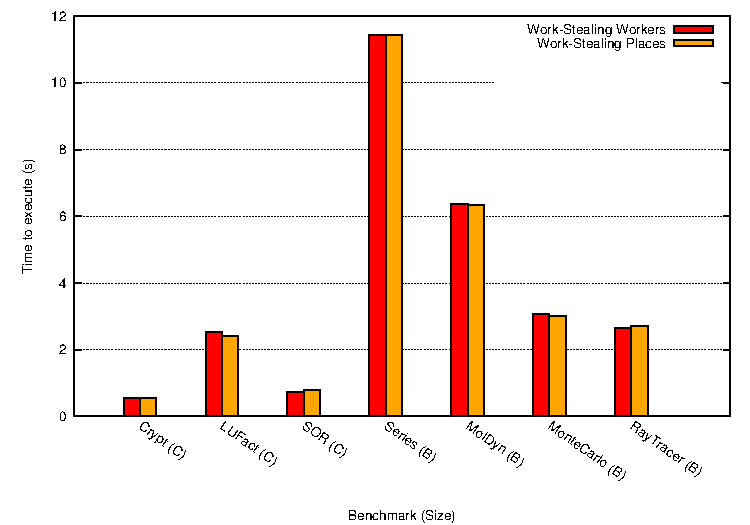
\includegraphics[width=0.85\textwidth]{figures/mafushi-jgf}
  \end{center}
\end{frame}

\note{
  \begin{itemize}
  \item It is important that our new scheduler implementation does not
    affect the performance of existing locality-ignorant intervals
    applications. Thus, we run the locality-ignorant JGF benchmarks
    with our new scheduler implementation.
  \item As the figure shows, the performance of the locality-ignorant
    JGF benchmarks executed on LASSI is comparable to the original
    implementation.
  \end{itemize}
}

\subsection{Locality Benchmarks}

% \begin{frame}{Cache Stress Test}
%   \begin{itemize}
%   \item Ported over from the threaded implementation
%   \item Randomly initializes two integer arrays of size 8 MB
%   \item Inline root interval produces 64 subintervals
%     \begin{itemize}
%     \item[$\rightarrow$] 32 with locality for \emph{place 0}, 32 for
%       \emph{place 1}
%     \end{itemize}
%   \item Half of the intervals work with array 0, the other half with
%     array 1
%   \item Each interval's task adds and multiplies all the elements of
%     its array 100 times
%   \end{itemize}
% \end{frame}

% \note{
%   \begin{itemize}
%   \item We ported the \emph{Cache Stress Test} benchmark from the
%     threaded to use intervals.
%   \item Like the threaded version, it first randomly initializes two
%     integer arrays of equal size to the last level cache per
%     processor.
%   \item Then it creates an inline root interval which produces 64
%     subintervals with their locality set to a specific place: 32 have
%     their locality set for \emph{place 0} and 32 for \emph{place 1}.
%   \item One half of the subintervals operate on the elements of the
%     first array and the other half operate on the elements of the
%     second array.
%   \item Each interval's task adds and multiplies all the elements of
%     its respective array 100 times.
%   \end{itemize}
% }

\begin{frame}{Cache Stress Test: Best and Worst Locality}
  \begin{columns}[c]
    \begin{column}{0.50\textwidth}
      \begin{center}
        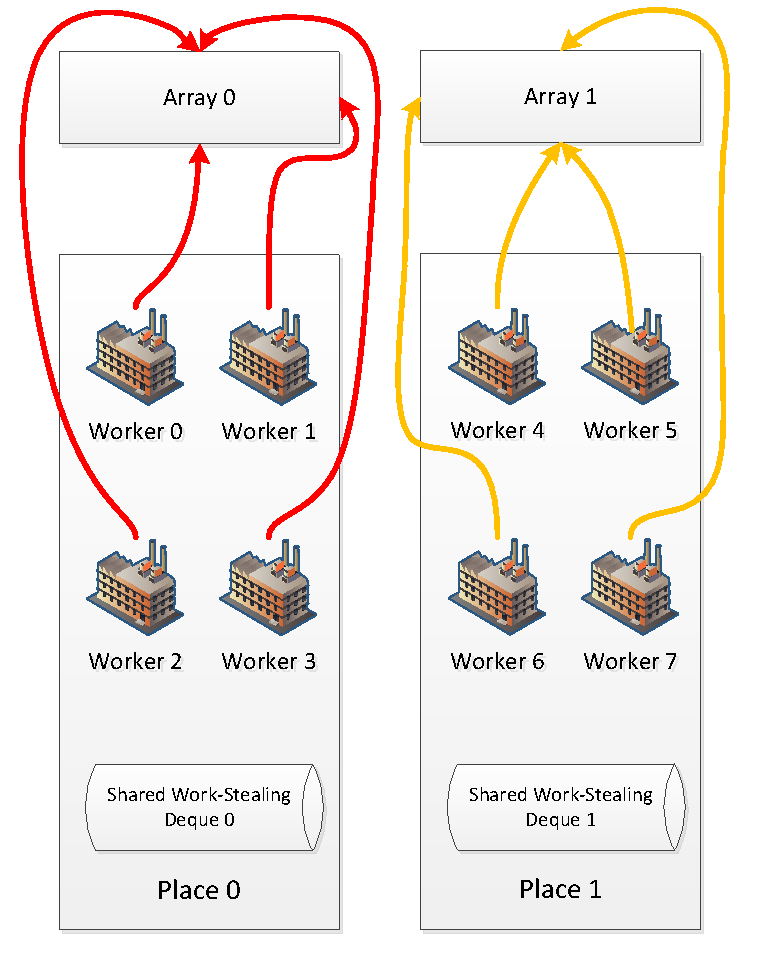
\includegraphics[width=\textwidth]{figures/cache-stress-test-mafushi-best} \\
        \tiny{Best locality}     
      \end{center}
    \end{column}
    \begin{column}{0.50\textwidth}
      \begin{center}
        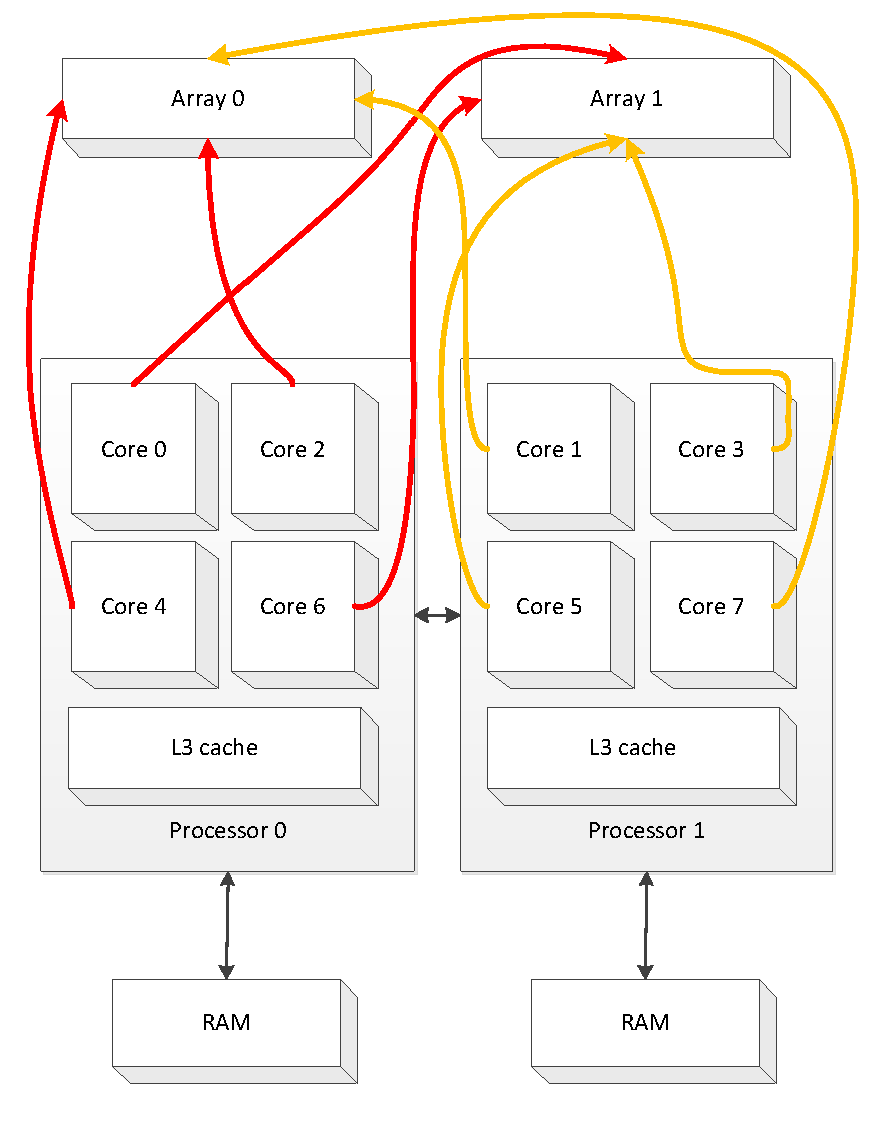
\includegraphics[width=\textwidth]{figures/cache-stress-test-mafushi-worst} \\
        \tiny{Worst locality}
      \end{center}
    \end{column}
  \end{columns}
\end{frame}

\note{ 
  The \emph{Cache Stress Test} benchmark was ported over from the
  threaded implementation. We wrote several variants, each having
  different locality properties. The figure illustrates \emph{Best}
  and \emph{Worst Locality}:

  \begin{itemize}
  \item In the \emph{Best Locality} all the intervals working on the
    first array have their locality set to \emph{place 0} and all
    intervals working on the second array have their locality set to
    \emph{place 1}.
  \item When using \emph{Worst Locality} half the intervals with
    locality for \emph{place 0} work on the first array, and the other
    half work on the second array and vice versa for the intervals
    with locality for \emph{place 1}.
  \end{itemize}
}

\begin{frame}{Cache Stress Test: Performance}
  \begin{itemize}
  \item \emph{Best locality} has speedup of up to $1.12\times$
  \item \emph{Best locality} benchmark has up to $1.5\times$ more L3
    cache read hits and $3.1\times$ fewer read misses:
  \end{itemize}

  \vspace{\stretch{1}}

  \begin{columns}[c]
    \begin{column}{0.5\textwidth}
      \begin{center}
        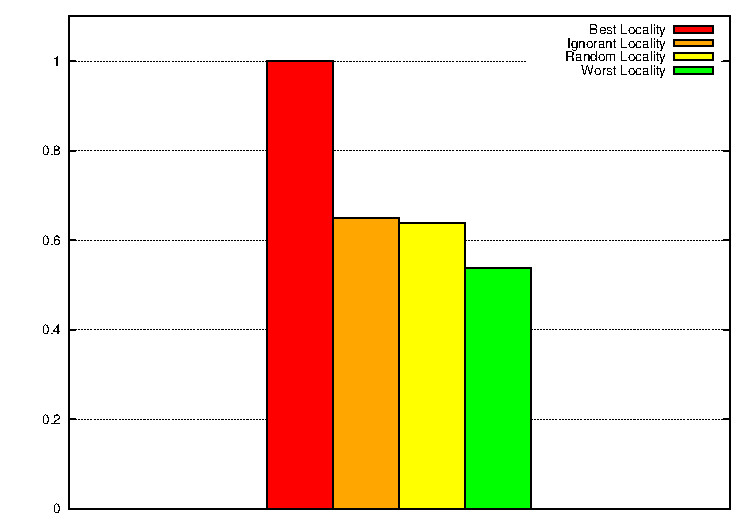
\includegraphics[width=\textwidth]{figures/cache-stress-test-cache-hits} \\
        \tiny{Cache read hits normalized to \emph{best locality}}
      \end{center}
    \end{column}
    \begin{column}{0.5\textwidth}
      \begin{center}
        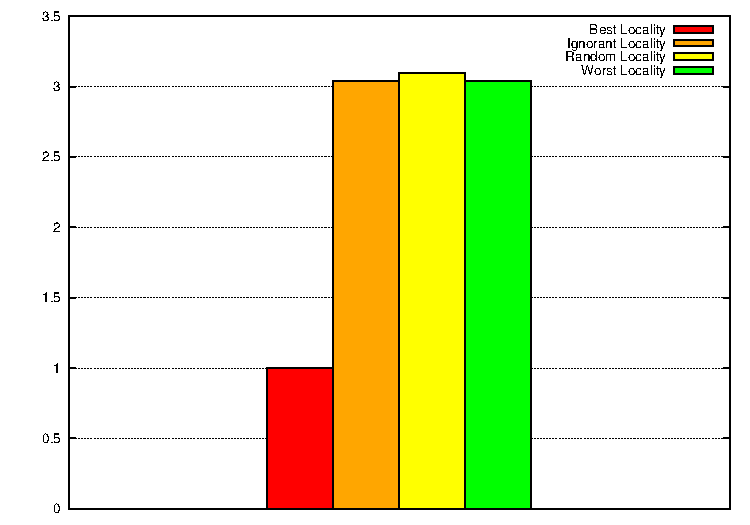
\includegraphics[width=\textwidth]{figures/cache-stress-test-cache-misses} \\
        \tiny{Cache read misses normalized to \emph{best locality}}
      \end{center}
    \end{column}
  \end{columns}
\end{frame}

\note{
  \begin{itemize}
  \item When running the intervals implementations of the \emph{Cache
      Stress Test} benchmarks, we observe similar behavior to the
    threaded versions. The \emph{best locality} implementation is
    about 12 percent faster compared to the other locality benchmarks.
  \item The \emph{best locality} benchmark has up to 50 percent more
    L3 cache read hits and 310 percent fewer cache read misses than
    the other benchmarks.
  \end{itemize}
}

\begin{frame}{Merge Sort}
  \begin{itemize}
  \item Uses divide-and-conquer to recursively sort \numprint{4194304}
    randomly initialized integer values
    \begin{itemize}
    \item[$\rightarrow$] Needs about 16 MB of memory
    \end{itemize}
  \item Creates \numprint{8192} sorter intervals per worker
  \item Each sorter randomly initializes array of size
    $\numprint{4194304} / (8 \times \numprint{8192})$ and sorts it
    sequentially
  \item Mergers merge two neighboring sorted arrays into one sorted
    array until all subarrays are merged into a single array
  \end{itemize}
\end{frame}

\note{
  \begin{itemize}
  \item The \emph{Merge Sort} benchmark uses divide-and-conquer to
    recursively sort randomly initialized integer values.
  \item The integer values need about 16 MB of memory which is equal
    to the size of the last level caches of our test machine.
  \item \emph{Merge Sort} first creates \numprint{8192} sorter
    intervals per worker.
  \item Each sorter randomly initializes an array of the size
    mentioned on the slide and sorts it sequentially
  \item Merger intervals merge two neighboring sorted arrays into one
    sorted array of doubled size until all subarrays are merged into a
    single array.
  \end{itemize}
}

\begin{frame}{Merge Sort: Locality}
  \begin{center}
    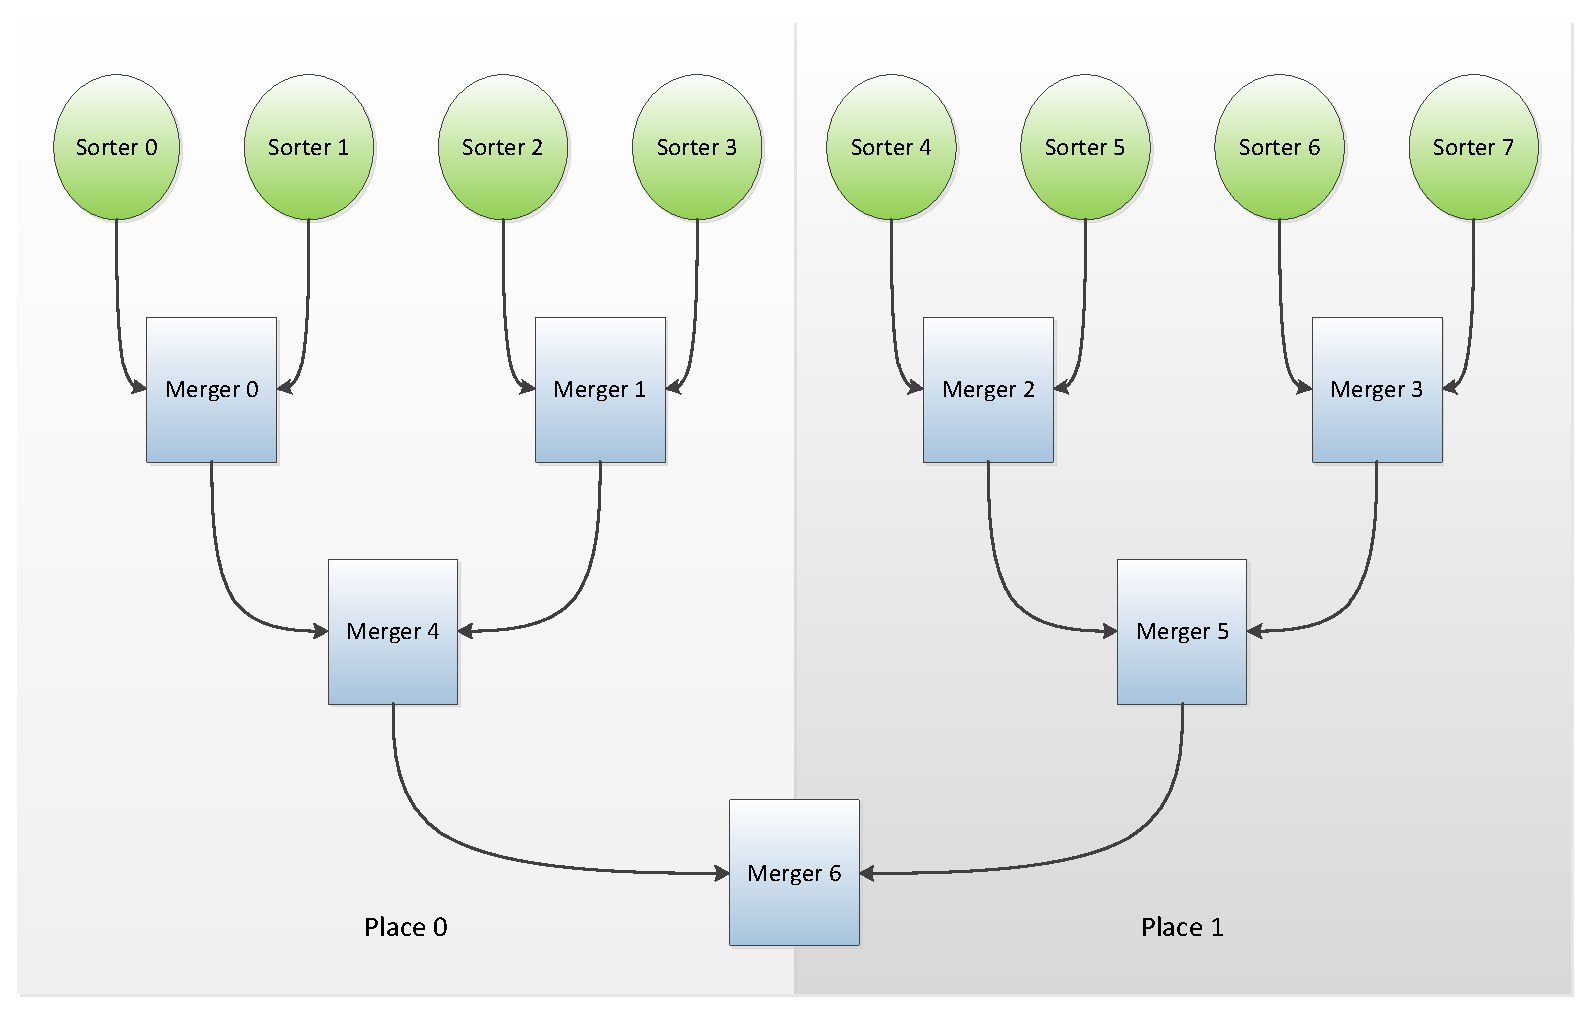
\includegraphics[width=\textwidth]{figures/mergesort-best-locality} \\
    \tiny{Best locality}    
  \end{center}
\end{frame}

\note{
  We implement several variants of the benchmark, each having
  different locality properties:

  \begin{itemize}
  \item The \emph{best locality} implementation puts data sharing
    intervals onto the same \emph{place}. Half the sorter intervals
    have locality for \emph{place 0} and the other half have their
    locality set for \emph{place 1}. Merger intervals are scheduled on
    the same place as their left predecessors in the tree hierarchy.
  \item When using \emph{Worst Locality}, the sorter intervals have
    the same locality as in the \emph{best locality}
    implementation. The merger intervals set their locality to the
    other place as their left predecessor in the tree hierarchy.
  \item In the \emph{Ignorant Locality} variant the sorter and merger
    intervals have no locality set.
  \end{itemize}

  The figure shows the place allocations for the benchmark variant
  with \emph{best locality}.
}

\begin{frame}{Merge Sort: Performance}
  \begin{columns}[c]
    \begin{column}{0.49\textwidth}
      \begin{itemize}
      \item \emph{Best locality} has speedup of up to $1.1\times$
      \item \emph{Best locality} benchmark has up to $1.02\times$ more
        L3 cache read hits and $1.07\times$ fewer read misses:
        \begin{itemize}
        \item[$\rightarrow$] Rather small benchmark size and limited
          level of data sharing
        \end{itemize}
      \end{itemize}
    \end{column}
    \begin{column}{0.51\textwidth}
      \begin{center}
        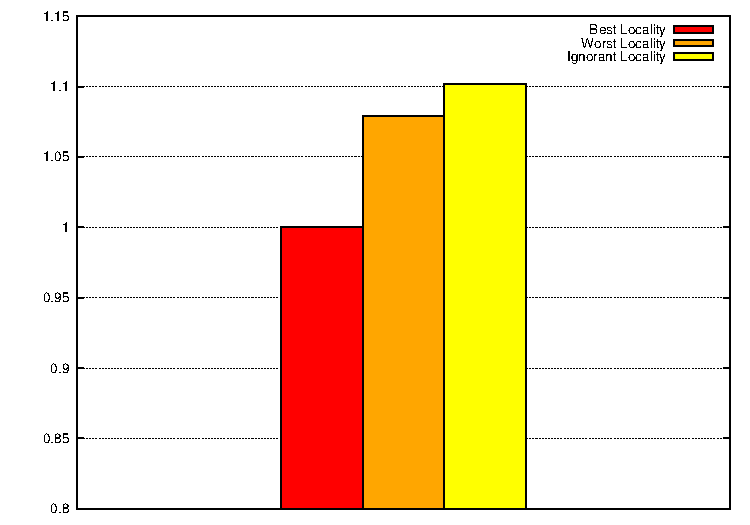
\includegraphics[width=\textwidth]{figures/mergesort} \\
        \tiny{Execution times normalized to \emph{best locality}}
      \end{center}
    \end{column}
  \end{columns}
\end{frame}

\note{
  \begin{itemize}
  \item The figure illustrates the execution times normalized to that
    of the \emph{best locality} implementation. The \emph{best
      locality} implementation provides a speedup of up to 10 percent
    compared to the other locality benchmarks.
  \item The difference between the number of cache read hits and
    misses is small: The \emph{best locality} variant has just about
    2\% more cache read hits and 7\% less cache read misses than the
    \emph{worst} and \emph{ignorant locality} variants:
    \begin{itemize}
    \item[$\rightarrow$] This is mainly because of the rather small
      benchmark size and limited level of data sharing between the
      intervals.
    \end{itemize}
  \end{itemize}
}

\begin{frame}{Block Matrix Multiplication}
  Multiplies two random $2048 \times 2048$ matrices $A$ and $B$ using the
  recursion:

  \begin{eqnarray*}
    \begin{pmatrix}
      C_{00} & C_{01} \\
      C_{10} & C_{11}
    \end{pmatrix}
    &
    =
    &
    \begin{pmatrix}
      A_{00} & A_{01} \\
      A_{10} & A_{11}
    \end{pmatrix}
    \cdot
    \begin{pmatrix}
      B_{00} & B_{01} \\
      B_{10} & B_{11}
    \end{pmatrix}
    \\[0.1cm]
    &
    =
    &
    \begin{pmatrix}
      A_{00} \cdot B_{00} + A_{01} \cdot B_{10} & A_{00} \cdot B_{01} + A_{01} \cdot B_{11} \\
      A_{10} \cdot B_{00} + A_{11} \cdot B_{10} & A_{10} \cdot B_{01} + A_{11} \cdot B_{11} \\
    \end{pmatrix}
  \end{eqnarray*}

  \vspace{\stretch{1}}

  \begin{itemize}
  \item[$\Rightarrow$] Matrix multiplication can be reduced to 8
    multiplications and 4 additions of $(n/2) \times (n/2)$
    submatrices
  \item[$\Rightarrow$] 8 multiplications can be calculated in parallel
    and when done, 4 additions can also be computed in parallel
  \end{itemize}
\end{frame}

\note{
  \begin{itemize}
  \item The \emph{Block Matrix Multiplication} benchmark multiplies
    two random $2048 \times 2048$ matrices. Each matrix needs about 16
    MB of memory and should just about fit in the L3 cache of the two
    processors of our test machine.
  \item We are using the recursion, thus the matrix multiplication can
    be reduced to 8 multiplications and 4 additions of $(n/2) \times
    (n/2)$ submatrices. The 8 multiplications can be calculated in
    parallel and when they are done, the 4 additions can also be
    computed in parallel.
  \end{itemize}
}

\begin{frame}{Block Matrix Multiplication: Locality}
  \begin{columns}[c]
    \begin{column}{0.31\textwidth}
      \begin{center}
        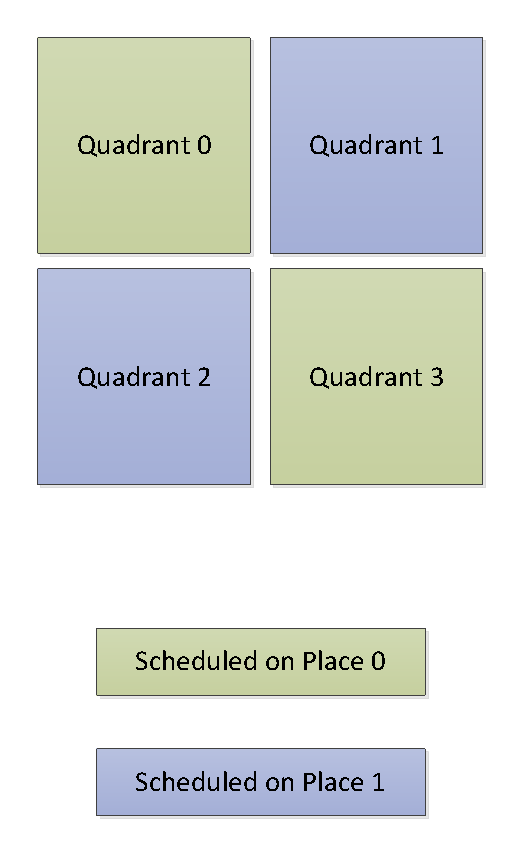
\includegraphics[width=\linewidth]{figures/matmult-best-locality} \\
        \tiny{Best locality}
      \end{center}
    \end{column}
    \begin{column}{0.31\textwidth}
      \begin{center}
        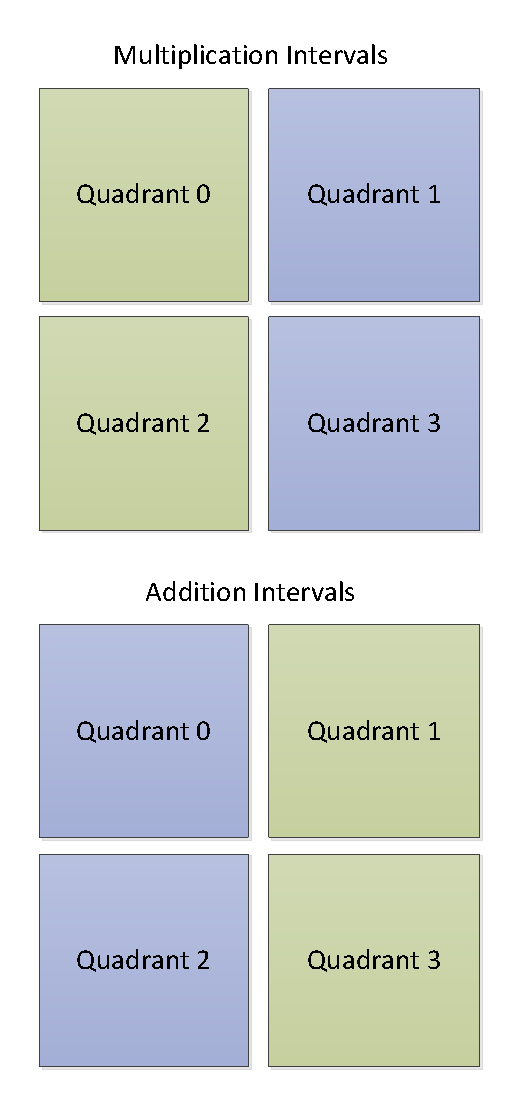
\includegraphics[width=\linewidth]{figures/matmult-worst-locality} \\
        \tiny{Worst locality}
      \end{center}
    \end{column}
  \end{columns}
\end{frame}

\note{
  We implement two variants of the benchmark, \emph{best locality} and
  \emph{worst locality}:

  \begin{itemize}
  \item The \emph{best locality} benchmark runs all addition and
    multiplication intervals of the submatrices of quadrants 0 and 3
    in \emph{place 0} and the ones of the quadrants 1 and 2 in
    \emph{place 1}. This way the places are able to share their local
    L3 cache in an efficient way.
  \item The \emph{worst locality} benchmark runs the multiplication
    and addition intervals in different places, destroying cache
    locality.
  \end{itemize}

  The figure illustrates the division of matrix quadrants between
  places for both variants.
}

\begin{frame}{Block Matrix Multiplication: Performance}
  \begin{columns}[c]
    \begin{column}{0.49\textwidth}
      \begin{itemize}
      \item \emph{Best locality} has speedup of up to $1.07\times$
      \item \emph{Best locality} benchmark has up to $1.02\times$ more
        L3 cache read hits and $1.06\times$ fewer read misses:
        \begin{itemize}
        \item[$\rightarrow$] Rather small benchmark size and limited
          level of data sharing
        \end{itemize}
      \end{itemize}
    \end{column}
    \begin{column}{0.51\textwidth}
      \begin{center}
        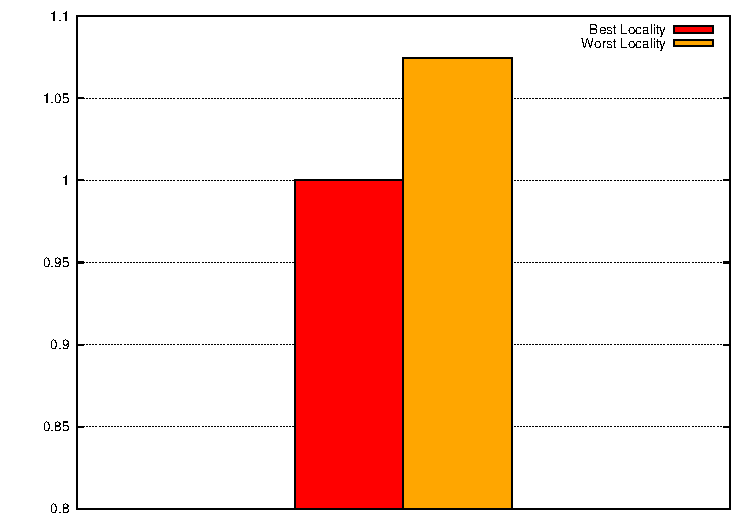
\includegraphics[width=\textwidth]{figures/matmult} \\
        \tiny{Execution times normalized to \emph{best locality}}
      \end{center}
    \end{column}
  \end{columns}
\end{frame}

\note{
  \begin{itemize}
  \item The figure depicts the execution time of the \emph{worst
      locality} implementation normalized to that of the \emph{best
      locality} implementation. The \emph{best locality}
    implementation shows a speedup of about 7\%.
  \item The difference between the number of cache read hits and
    misses is little: The \emph{best locality} variant has just about
    2\% more cache read hits and 6\% less cache read misses than the
    \emph{worst locality} variant.
    \begin{itemize}
    \item[$\rightarrow$] The main reason for this is the rather small
      benchmark size and limited level of data sharing between the
      intervals.
    \end{itemize}
  \end{itemize}
}


\section{Conclusions and Future Work}

\begin{frame}{Outline}
  \tableofcontents[current]
\end{frame}

\note{}

\begin{frame}{Conclusions}
  \begin{itemize}
  \item Introduced LASSI, a locality-aware scheduler for intervals
  \item \emph{Work-Stealing Places} to support locality-awareness
  \item Performance of existing locality-ignorant programs comparable
    to the original scheduler implementation
  \item Scheduling data sharing intervals on the same processor:
    \begin{itemize}
    \item[$\rightarrow$] Prefetching of shared regions for one another
    \end{itemize}
  \item Benchmarks do not test scheduling non-communicating intervals
    with high memory footprints on different processors
  \end{itemize}
\end{frame}

\note{
  \begin{itemize}
  \item In this thesis, we introduced LASSI, a locality-aware
    scheduler for intervals using locality hints provided by the
    programmer.
  \item Instead of employing work-stealing workers, LASSI uses
    \emph{Work-Stealing Places} to provide locality-awareness.
  \item The performance of existing locality-ignorant programs run
    with LASSI is comparable to the original scheduler implementation.
  \item By scheduling data sharing intervals on the same processor
    they perform prefetching of shared regions for one another which
    improves performance. Our experimental results show a speedup as
    well as an increase in L3 cache read hits and a decrease in cache
    read misses.
  \item Our benchmarks do not test how scheduling non-communicating
    intervals with high memory footprints on different processors
    helps to reduce cache contention and potential cache capacity
    problems.
  \end{itemize}
}

\begin{frame}{Future Work}
  \begin{itemize}
  \item Improve API of \emph{Work-Stealing Places} and locality-aware
    intervals
  \item Make underlying machine transparent to the user
  \item Extend \emph{Work-Stealing Places} to co-locate tasks and
    data
  \item Avoid counter-productive steals
  \item Online contention detection to dynamically reduce or increase
    number of worker threads depending on system load
  \end{itemize}
\end{frame}

\note{
  \begin{itemize}
  \item A possible area of future work would be to improve the
    API. Places have to be manually configured for each system. This
    should be automated by making the hardware transparent to the
    user.
  \item LASSI depends on the heuristics of the NUMA-aware allocator
    implemented in Java HotSpot VM to provide automatic memory
    placement optimizations. Further research could be done in
    extending \emph{Work-Stealing Places} to co-locate tasks and data.
  \item Load balancing across work-stealing places can lead to
    counter-productive stealing. Future work should avoid such steals.
  \item Worker threads share their assigned core with other processes
    in the system. Online contention detection could be used to
    dynamically reduce or increase the number of worker threads.
  \end{itemize}
}


\section*{Outro}

\begin{frame}
  \begin{center}
    \huge Questions?
  \end{center}
\end{frame}

\note{}


\appendix

\section{Appendix}

\subsection{Bibliography}

\begin{frame}
  \begin{thebibliography}{10}
    % Articles
    \beamertemplatearticlebibitems

  \bibitem{data-locality} Umut A. Acar et al. {\em``The data locality
      of work stealing''}. 2000.

  \bibitem{ws-sched} Robert D. Blumofe and Charles
    E. Leiserson. {\em``Scheduling multithreaded computations by work
      stealing''}. 1999.

  \bibitem{cilk} Robert D. Blumofe et al. {\em``Cilk: an efficient
      multithreaded runtime system''}. 1995.

  \bibitem{slaw} Yi Guo et al. {\em``SLAW: a scalable locality-aware
      adaptive work-stealing scheduler for multi-core
      systems''}. 2010.

  \bibitem{java-fork-join} Doug Lea. {\em``A Java fork/join
      framework''}. 2000.

  \bibitem{intervals} Nicholas D. Matsakis and Thomas
    R. Gross. {\em``Programming with Intervals''}. 2009.

  \bibitem{cache-affinity} M. S. Squillante and
    E. D. Lazowska. {\em``Using Processor-Cache Affinity Information
      in Shared-Memory Multiprocessor Scheduling ``}. 1993.

  \bibitem{cmp} Bratin Saha et al. {\em``Enabling scalability and
      performance in a large scale CMP environment''}. 2007.

  \end{thebibliography}
\end{frame}

\note{}

\subsection{Additional Material}

\begin{frame}[fragile]{Intel Nehalem Test Machine}
  \begin{columns}[c]
    \begin{column}{0.57\textwidth}
      \begin{itemize}
      \item Intel Nehalem with 2 processors and 4 cores each
      \item Ubuntu 9.04 with kernel 2.6.29 patched to support perfmon2
      \item Sun Hotspot JDK 1.6.0\_20 invoked with:
        \begin{lstlisting}[basicstyle=\fontsize{8}{9}\selectfont\ttfamily]
  -server -Xmx4096M -Xms4096M
  -Xss8M -XX:+UseNUMA
        \end{lstlisting}
      \item perfmon2 tracks:
        \begin{itemize}
        \item \lstinline!UNC_LLC_HITS.READ!: Number of L3 cache read
          hits
        \item \lstinline!UNC_LLC_MISS.READ!: Number of L3 cache read
          misses
        \end{itemize}
      \end{itemize}
    \end{column}
    \begin{column}{0.43\textwidth}
      \begin{center}
        \includegraphics[width=\textwidth]{figures/mafushi-setup}
      \end{center}
    \end{column}
  \end{columns}
\end{frame}

\note{
  \begin{itemize}
  \item The performance results are obtained on an Intel Nehalem
    system with 2 processors and 8 cores, running Ubuntu with kernel
    patched to support perfmon2.
  \item The JVM used is Sun Hotspot which is invoked with the listed
    parameters.
  \item Besides the runtime of the benchmarks, we are mostly
    interested in the count of cache hit and miss events. Since the
    last level cache is part of the uncore, we have to use the uncore
    PMU to count L3 cache events.
  \item The execution times and cache event counts reported are the
    average of the 3 best benchmark iterations from 10 separate
    invocations.
  \end{itemize}
}

\subsection{Work-Stealing Queue Implementations}

\begin{frame}{Alternative Work-Stealing Queues}
  \begin{itemize}
  \item Performance of work-stealing schedulers in large part
    determined by the efficiency of the work queue
  \item Non-blocking queues employ atomic synchronization primitives
    such as Compare-and-Swap instead of mutual exclusion
  \item Current work-stealing queue of intervals uses mutual exclusion
    when trying to steal
  \end{itemize}

  \vspace{\stretch{1}}

  \begin{itemize}
  \item[$\Rightarrow$] Design and explore alternative non-blocking
    queues with the aim of improving work-stealing performance
  \end{itemize}
\end{frame}

\note{
  \begin{itemize}
  \item The performance of work-stealing schedulers is in a large part
    determined by the efficiency of their work queue
    implementations.
  \item In the non-blocking work-stealing scheduler, the
    queues are implemented with non-blocking synchronization. That is,
    instead of using mutual exclusion, it uses atomic synchronization
    primitives such as Compare-and-Swap.
  \item The current work-stealing queue of intervals however uses
    mutual exclusion when trying to steal.
  \item Thus, as a separate effort, we design and explore alternative
    non-blocking queue implementations with the aim to improve
    work-stealing performance.
  \end{itemize}
}

\begin{frame}{Results}
  \begin{itemize}
  \item Evaluate the performance of our queues with intervals
    implementations of various Java Grande Forum benchmarks
  \item None of the alternative work-stealing queues significantly
    improves performance on our test machines
  \end{itemize}

  \vspace{\stretch{1}}

  \begin{block}{Possible Reason}
    There is no noticeable difference between the speedup of
    work-stealing and a global shared work queue when not using more
    than 8 cores
  \end{block}
\end{frame}

\note{
  \begin{itemize}
  \item Our hypothesis was that we could improve the performance of
    the intervals scheduler with non-blocking work-stealing queues.
  \item We evaluated the performance of our alternative queues by
    using the intervals implementations of various Java Grande Forum
    benchmarks.
  \item None of the work-stealing queues we developed significantly
    improves work-stealing performance on the machines we had to test
    them with.
  \item Apart from the more complex implementation in comparison to
    the original \emph{Work-Stealing Deque}, a possible reason for
    this could be the rather small number of cores of our benchmark
    machines. We could not find any significant difference between the
    runtimes of the Java Grande Forum benchmarks when using the
    different implementations -- whether we use work-stealing or a
    single shared work queue, we get almost the same results.
  \end{itemize}
}

\begin{frame}{Future Work}
  \begin{itemize}
  \item Explore the performance of the different work-stealing queues
    on machines with more than 8 cores
  \item See how our work-stealing queues would benefit from using the
    steal-half algorithm of Hendler and Shavit
  \item Using a shared pool of arrays:
    \begin{itemize}
    \item When the queue needs a larger array, allocate one of the
      appropriate size from the pool
    \item Whenever it shrinks to a smaller array and does not need the
      larger array anymore, return it to the pool
    \end{itemize}
  \end{itemize}
\end{frame}

\note{
  \begin{itemize}
  \item Given the results of the performance evaluation, a direction
    for future research would be to explore the performance of the
    different work-stealing queue implementations on machines
    featuring more than 8 cores.
  \item It may also be interesting to see how our work-stealing queues
    would benefit from using the steal-half algorithm of Hendler and
    Shavit.
  \item Another optimization would be working with a shared pool of
    arrays. With the shared pool implementation, whenever the queue
    needs a larger array, it allocates one of the appropriate size
    from the pool, and whenever it shrinks to a smaller array and does
    not need the larger array anymore, it can return it to the pool.
  \end{itemize}
}

\end{document}
